%!TEX root = ../thesis.tex
\begin{savequote}[75mm]
\hl{If a team couldn’t be fed with two pizzas, it was too big.}
\qauthor{Jeff Bezos}
\end{savequote}

% https://areomagazine.com/2019/04/10/agile-and-the-software-industrys-ideology-problem/ 
%https://www.softwaretestinghelp.com/agile-manifesto/
%https://www.smartsheet.com/comprehensive-guide-values-principles-agile-manifesto

\chapter{Agile Software Development}
\label{chapter_3}

Before getting into the implementation and adaptation of Jira and Confluence, \hl{let's back up a little} and understand the concept of Agile, a Software Development Life Cycle (or SDLC) model.\\
%todo rivedere per bene
SDLCs did not emerge until the 1960s; they are considered to be the oldest formalization of framework.
%The Space Shuttle program, which operationally launched in 1982, used information and processing technologies from the 1960s.
A SDLC refers to the ensemble of activities that compose a software project.\\
It starts with the concepts of understanding the problem as well as the requirements and it ends with the retirement of the system (when there is no more maintenance) or with the cancellation of the project.\\
Small projects (generally for a single person) have a simpler life \hl{cycle: find the problem and write a program to solve it: once the problem has been solved}, the program can be deleted and forgotten.\\
%todo or in larger problems / solved
In larger projects, that require a team to be developed, there must be some explicit rules to set a higher quality for the software.\\
As activities are assigned to different people, it becomes critical that all participants share a common view of the execution of the project.
A SDLC model is a framework providing the ordering and dependencies of life cycle activities, managing these can be a major impact for a successful project and its duration.\\
For example, a change in requirements during implementation may invalidate a substantial amount of work and delay the delivery of the system by several months.
Different life cycle models prescribe different actions to handle such changes\cite{software_lyfe_cycle}.\\
%https://en.wikipedia.org/wiki/Software_development_process
%todo mettere tra virgolette
There are many SDLCs like Waterfall, Prototyping, Iterative and Incremental Development, Spiral Development, Rapid Application Development, and Extreme Programming. (XP). 
%todo modificare immagine
%Font piccolo nell'immagine e nella didascalia. In principio, il font dovrebbe essere a grandezza costante sia nel testo che nelle immagini
\begin{figure}[H]
	\centering
	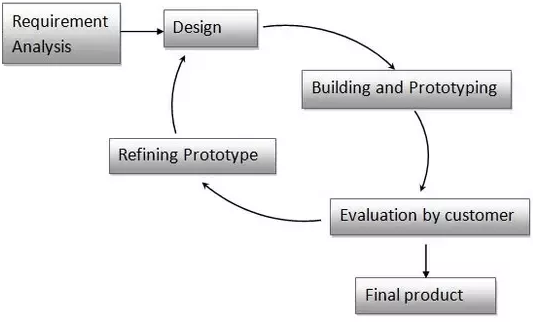
\includegraphics[width=.7\textwidth]{resources/prototype}\\
	\caption{The Prototype model}
\end{figure}
\begin{figure}[H]
	\centering
	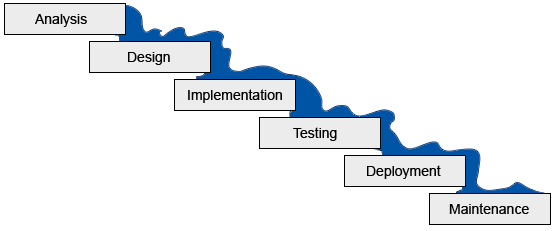
\includegraphics[width=.7\textwidth]{resources/warterfall}\\
	\caption{The Waterfall model}
\end{figure}
%https://www.iso.org/obp/ui/#iso:std:iso-iec:tr:24774:ed-2:v1:en
%todo citare https://www.iso.org/standard/53815.html !!
As the word \Quote{model} suggests, each company may have its own SDLC designed ad hoc for their internal use.\\
This led to the creation of a standard that presents the guidelines for the elements that are most frequently used in describing a process: the title, purpose, outcomes, activities, task and information item.
%todo citare
The ISO/IEC TR 24774:2010: Systems and software engineering -- Life cycle management -- Guidelines for process description\cite{iso_53815}.\\
The complexity and slowness in producing a concrete product in older SDLCs brought the need for a faster and more communicative model.\\
%https://www.tutorialspoint.com/sdlc/sdlc_agile_model.htm
%todo mettere a glossario
%Agile SDLC model is a combination of iterative and incremental process models with focus on process adaptability and customer satisfaction by rapidly and continuously deliver of working software product.
%todo trovare immagine a risoluzione migliore
\begin{figure}[H]
	\centering
	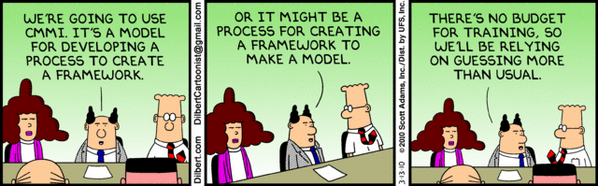
\includegraphics[width=\textwidth]{resources/BffFTn_CAAAEvGn}\\
	\caption{\textit{Redmine}'s logo}
\end{figure}
This chapter describes the most fundamental points of the Agile method, how it started and the adaptations that derived from it, like Scrum.
At the end, it also explains how Athonet's adaptation of the Agile life cycle works.

\section{The need for a new Software Life Cycle}
	The decade of 1990 represented a very important turning point for the digital industry.
	Computers were spreading everywhere and the software companies faced the so-called application development crisis.\\
	The problem was that businesses moved too fast and within the space of three years, requirements, systems, and even entire businesses were likely to change. 
	It meant that a lot of software ended up being incomplete or canceled halfway and the ones that made it through, even if they fulfilled the original objectives of the client, may not meet all the business needs\cite{agility-beyond-history}.
%	https://hackr.io/blog/sdlc-methodologies
	SDLC models can be of two types:
	\begin{itemize}
		\item Iterative: enhances the evolving versions until the complete system is implemented and ready to be deployed
		\item Incremental: the product is designed, implemented and tested incrementally until it is finished
	\end{itemize}
	One of the most characteristic models used before Agile was the Sequential model (or Waterfall).
	The waterfall model became very famous because it has many strong points as:
	\begin{itemize}
		\item Uses clear structure
		\item Determines the end goal early
		\item Transfers information well
	\end{itemize}
	On the other hand, it became obsolete when projects started to be more dynamic and complex.
	Some of it's disadvantages are:
	\begin{itemize}
		\item Makes changes difficult
		\item Excludes the client and/or end user
		\item Delays testing until after completion
	\end{itemize}
	The excessive documentation, the forceful binding to the unchangeable decisions made early in the project and the little communication with the client brought to the need of a new model that prioritizes the product and the stakeholders over bureaucracy.\\
	Those things frustrated people like Jon Kern, an aerospace engineer in the 1990s that with other figures from different industries \Quote{were looking for something that was more timely and responsive}, as he noted.
	He was one of 17 software leaders that started meeting informally and talking about ways to develop software in a simpler way without the excess of documentation and other strict rules.\\
	These talks led to the now famous Snowbird meeting (in Utah, February 2001), when the Agile Manifesto was written down and published.

%
\section{The Agile manifesto}
	The Agile Manifesto is a brief document built on four foundational values and twelve supporting principles for Agile software development\cite{agilemanifesto}.\\
	The four values written on the official website\cite{agile_official} are:
	\begin{itemize}
		\item \textbf{Individuals and interactions} over processes and tools
		\item \textbf{Working software} over comprehensive documentation
		\item \textbf{Customer collaboration} over contract negotiation
		\item \textbf{Responding to change} over following a plan
	\end{itemize}
	The responsiveness of people and embracing the importance of changes are the fundamentals of Agile.
	Although documentation is secondary, it's important to note that Agile streamlines documentation and does not eliminate it.\\
	These twelve principles emphasize things like \Quote{early and continuous delivery of valuable software” and “continuous attention to technical excellence}, and are: 
	\begin{enumerate}
		\item Our highest priority is to satisfy the customer through early and continuous delivery of valuable software.
		\item Welcome changing requirements, even late in development. Agile processes harness change for the customer's competitive advantage.
		\item Deliver working software frequently, from a couple of weeks to a couple of months, with a preference to the shorter timescale.
		\item Business people and developers must work together daily throughout the project.	
		\item Build projects around motivated individuals. Give them the environment and support they need, and trust them to get the job done.
		\item The most efficient and effective method of conveying information to and within a development team is face-to-face conversation.
		\item Working software is the primary measure of progress.
		\item Agile processes promote sustainable development. The sponsors, developers, and users should be able to maintain a constant pace indefinitely.	
		\item Continuous attention to technical excellence and good design enhances agility.
		\item Simplicity--the art of maximizing the amount of work not done--is essential.
		\item The best architectures, requirements, and designs emerge from self-organizing teams.
		\item At regular intervals, the team reflects on how to become more effective, then tunes and adjusts its behavior accordingly.
	\end{enumerate}
	All of them are important but, in my opinion, the ones that add the most value to the Agile line of thought and that differentiate it from the other methods are 2, 4 and 6: they represent the intent of placing the product and the customer above everything else, allowing the use of small informal meetings (even if the decisions should be recorded) and the easy change of requirements because the client is always involved, even as an end user (tester).\\
	Each Agile methodology applies the four values in different ways.
	However, all of them rely on these values to guide the development and delivery of high-quality, working software\cite{4-values-of-the-agile-manifesto}.

\section{Agile's little big cousins}
	While Agile's manifesto contains values and principles, these are not prescriptive.
	In fact the manifesto does not outline specific processes, procedures or best practices.
	The goal is not to develop a rigid framework but rather create a mindset for software development.
	Agile is a blanket term that describes a set of software development principles.\\
	There are many methodologies that derive from Agile's thinking, the most famous ones, according to the annual survey\cite{state-of-agile} from VersionOne's team are:
	\begin{itemize}
		\item Scrum
		\item Scrumban
		\item Kanban
		\item Extreme Programming (XP)
	\end{itemize}
	The essence of Scrum is being agile (fast): a small team that is highly flexible and adaptive.
	\begin{figure}[H]
		\centering
		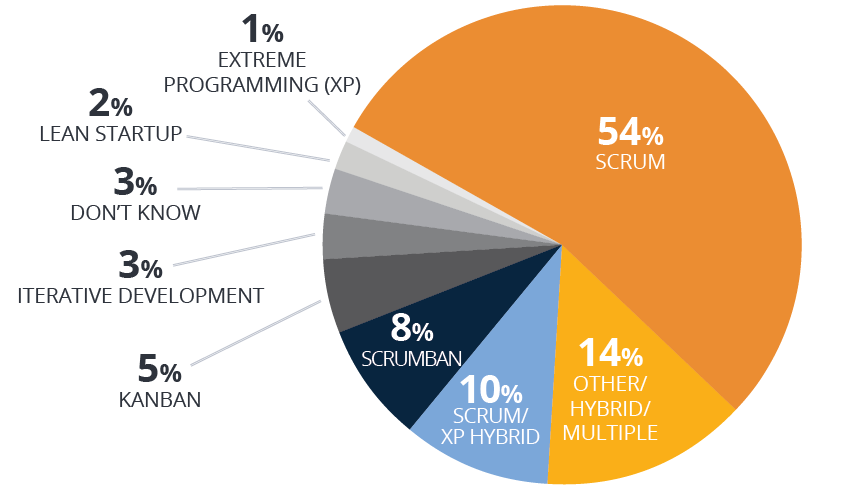
\includegraphics[width=.8\textwidth]{resources/agile-usage-chart}\\
		\caption{The Waterfall and Prototype SDLC models}
	\end{figure}

	%todo modificare immagine
	\begin{figure}[H]
		\centering
		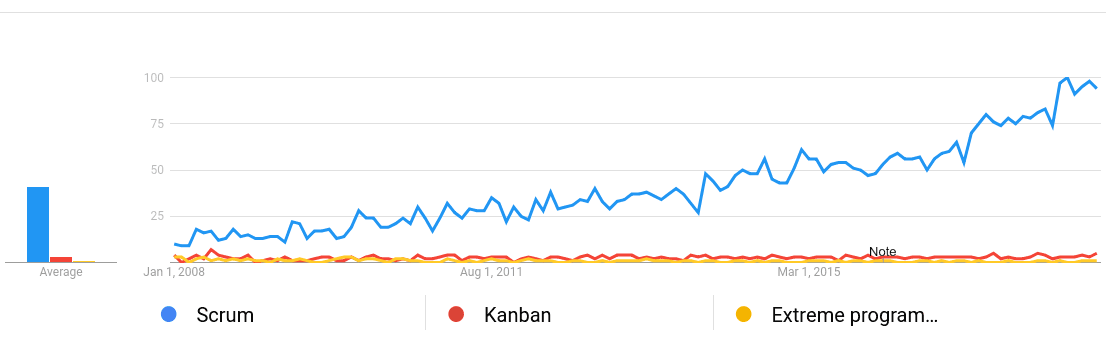
\includegraphics[width=\textwidth]{resources/trends}\\
		\caption{The Waterfall and Prototype SDLC models}
	\end{figure}
	This survey is quite interesting because it provides information from small and big real companies that want to share their experience.
	A very important fact to be noted is that although Technology companies are the ones that mostly participated to the survey, there are other industries that use Agile and are interested in sharing their experience.
	\begin{figure}[H]
		\centering
		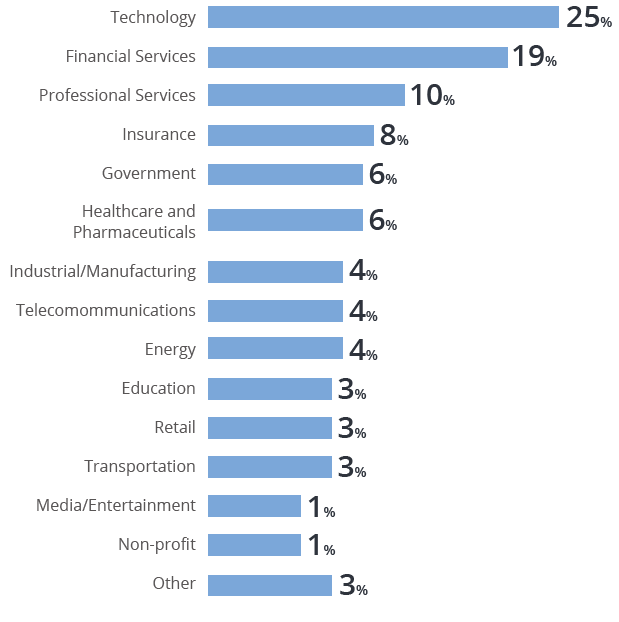
\includegraphics[width=.8\textwidth]{resources/Untitled_2}\\
		\caption{The Waterfall and Prototype SDLC models}
	\end{figure}
	It states that for the year 2018 (which marked their 13th annual report) the reasons for adopting Agile were productivity, improving team morale, reducing product risk (with a lesser percentage than the previous year) and about reducing project costs.\\
	The measures of success mostly cited by the respondents were customer, or user, satisfaction and business value.\\

	%todo Qui devi elencare, e mettere un link alla figura con le percentuali. Il testo dovrebbe contenere tutte le informazioni necessarie per capire il tuo discorso, e le figure servono come chiarimento. Ciascuna figura dovrebbe essere indipendente, nel senso che tra immagine e didascalia si dovrebbe riuscire a capire tutto. 

	According to these companies, the benefits of adopting Agile are:
	\begin{figure}[H]
		\centering
		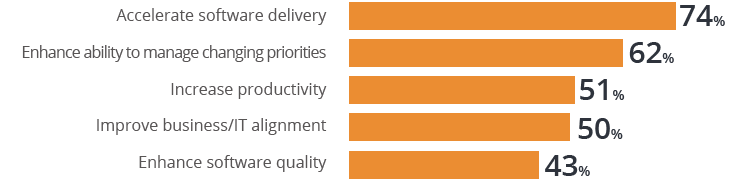
\includegraphics[width=.8\textwidth]{resources/Untitled}\\
		\caption{The Waterfall and Prototype SDLC models}
	\end{figure}

	Also the questionnaire contained a question about what are the recommended Agile project management tools.
	
	%todo modificare immagine
	\begin{figure}[H]
		\centering
		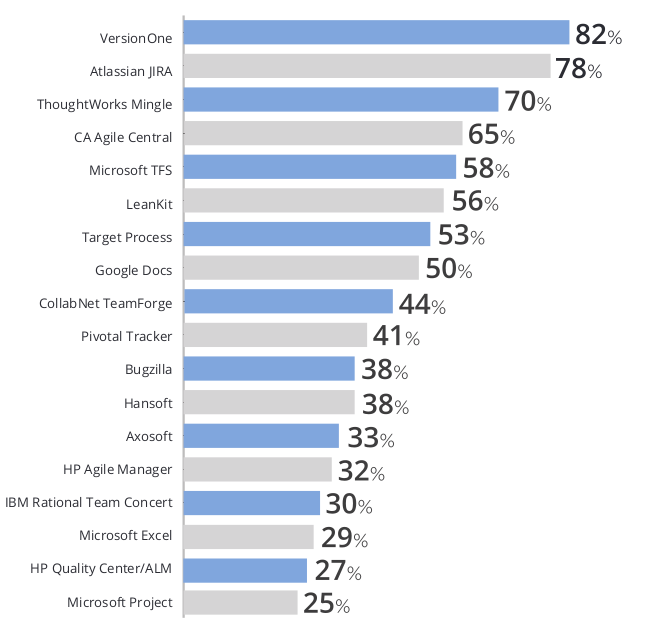
\includegraphics[width=.8\textwidth]{resources/Screenshot}\\
		\caption{The Waterfall and Prototype SDLC models}
	\end{figure}

	As we can see Jira is the second most recommended one.

	\begin{figure}[H]
		\centering
		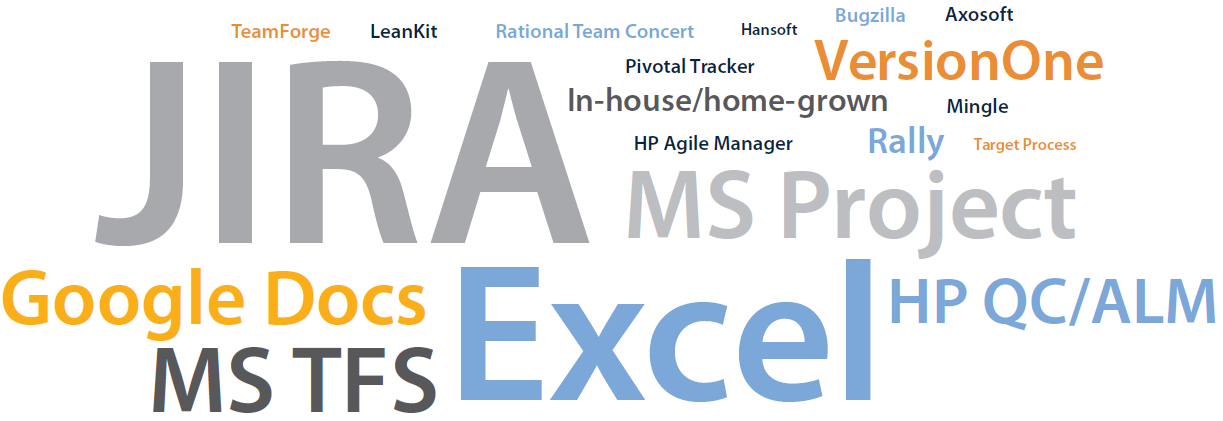
\includegraphics[width=.8\textwidth]{resources/Untitled_4}\\
		\caption{The Waterfall and Prototype SDLC models}
	\end{figure}

\section{Agile in practice}
\hl{Briefly describe how some companies use Agile: Spotify / Netflix / Amazon}

% SPOTIFY
%https://medium.com/@media_75624/exploring-key-elements-of-spotifys-agile-scaling-model-471d2a23d7ea
%https://medium.com/productmanagement101/spotify-squad-framework-part-i-8f74bcfcd761

% AMAZON
%https://www.forbes.com/sites/stevedenning/2019/06/02/how-amazon-became-agile/

% MICROSOFT
%https://www.forbes.com/sites/stevedenning/2015/10/27/surprise-microsoft-is-agile/

% NETFLIX
%https://smartbear.com/blog/develop/5-lessons-agile-teams-can-learn-from-netflix/
%http://www.agileadvice.com/2018/03/02/profiles/a-case-study-of-netflixs-high-performance-culture/

%LSD (Lean Software Development)
%This methodology is an adaptation of the Toyota lean manufacturing principles to software development. It was introduced in 2009 by Marry and Tom Poppendieck in their book "Lean Software Development: An Agile Toolkit."

\section{The roles in Agile}
	A distinctive characteristic of the Agile methodology is it's definition of roles: they are not positions, any given person takes on one or more roles and can switch them over time, and any given role may have zero or more people in it at any given point in a project\cite{agileRoles}.
	The ideal team is considered to be composed of five or six people.\\
	These roles are:
	\begin{itemize}
		\item Team leader: team coach or project lead in other methods (Scrum-master e.g.), he is responsible for facilitating the team, obtaining resources for it, and protecting it from problems
		\item Product owner: an executive or key stakeholder, the Product Owner has a vision for the end product and a sense of how it will fit into the company’s long-term goal
		\item Team member: developer or programmer, is responsible for the creation and delivery of a system
		\item Stakeholder: any other person that has direct or indirect interest in the project
	\end{itemize}

%https://www.dummies.com/careers/project-management/agile-project-management-artifacts/
%https://www.atlassian.com/agile/project-management/metrics
%https://www.cognizant.com/services-resources/Services/Cognizant-Agile-Metrics-What-You-Need-to-Want-to-and-Can-Measure.pdf
\section{Time cycles and metrics}
	Scrum teams coordinate development into time-boxed sprints.
	Outside the sprint, teams organize and forecast the amount of work that can be concluded.
	The goal is to have all the forecasted work completed by the end of the sprint.
	There are metrics used to track the completion of tasks, these are called burndown reports.
	\begin{figure}[H]
		\centering
		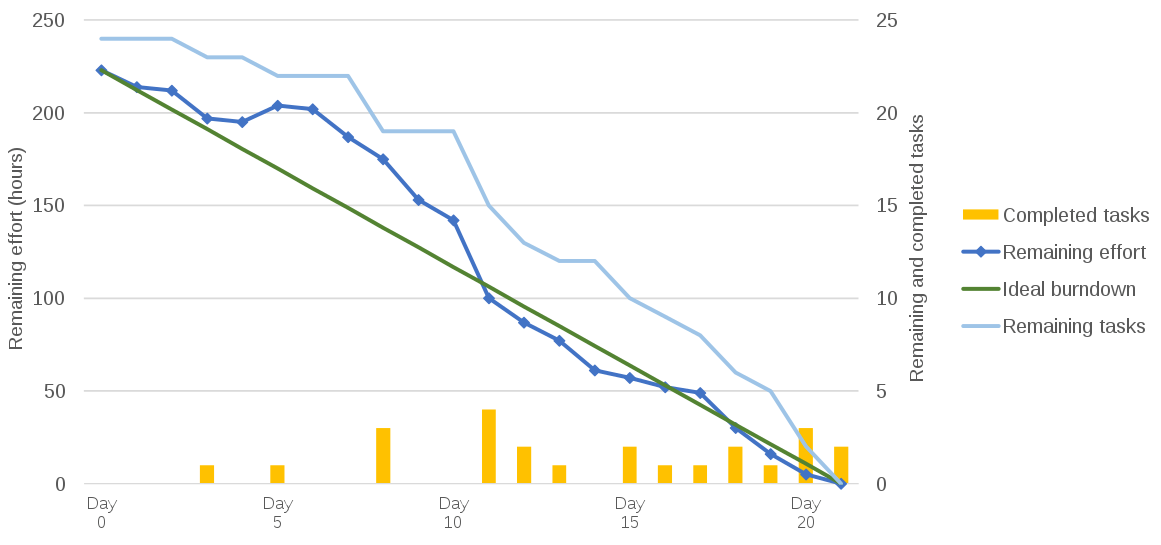
\includegraphics[width=\textwidth]{resources/burndown}\\
		\caption{The Waterfall and Prototype SDLC models}
	\end{figure}
	The x-axis represents time, and the y-axis refers to the amount of work left to complete, measured in either story points or hours.\\
	The sprint is one of the most important time periods in Agile, the other principal ones, according to Atlassian's Agile Coach\cite{epics-stories-themes} are:
	\begin{itemize}
		\item Stories: short requirements or requests written from the perspective of an end user
		\item Epics: large bodies of work that can be broken down into a number of smaller tasks (called stories)
		\item Initiatives: collections of epics that drive toward a common goal
		\item Themes: large focus areas that span the organization
	\end{itemize}
	\begin{figure}[H]
		\centering
		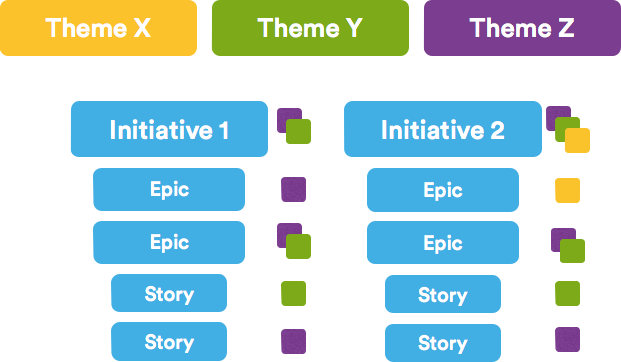
\includegraphics[width=\textwidth]{resources/Themes}\\
		\caption{The Waterfall and Prototype SDLC models}
	\end{figure}
	
%	todo prendere da questo sito https://www.atlassian.com/agile/project-management/epics-stories-themes
	
%https://leankit.com/learn/agile/what-are-the-disadvantages-of-agile/
\section{Disadvantages of Agile Software Development}
	Despite the benefits offered by the Agile model, transition a company's way of working to it is not that easy and if done wrong it may make damage instead of good.
	According to the American entrepreneur Adam Fridman, here are the drawbacks\cite{massive-downside-of-agile} of Agile:
	\begin{enumerate}
		\item Less predictability: developers may not be able to quantify the full extend of the required effort
		\item More time and commitment: a constant interaction, with many face-to-face conversations, is required
		\item Greater demands on developers and clients: extensive user involvement that impacts the quality and success of the project
		\item Lack of necessary documentation: new members that join the team may need more time to understand the project
		\item Project easily falls off track: if a consumer's feedback or communications are not clear, a developer might focus on the wrong areas of development
	\end{enumerate}
	
\section{What Agile variant Athonet uses}
	As many small companies, Athonet will not strictly use one Agile implementation.
	This is also due because of the nature of their product that is not released in simple software patches but it presents itself in a more monolithic version.
	After a research for the available software development life-cycle tools on the market, they chose to try Atlassian's Jira in tandem with Confluence.\\
	As I will say in \Chapref{chapter_5}, the managers liked the idea of Kanban because it allows the employees to come in the morning and choose what they want to work on from the backlog without giving them a two week period of time but letting them complete the tasks in time for the following release.
	But they also liked the idea of having a tool that could transition from a type of project to another in case they want to start applying stricter rules in the future.
	%todo immagine doppia modificare
	\begin{figure}[H]
		\centering
		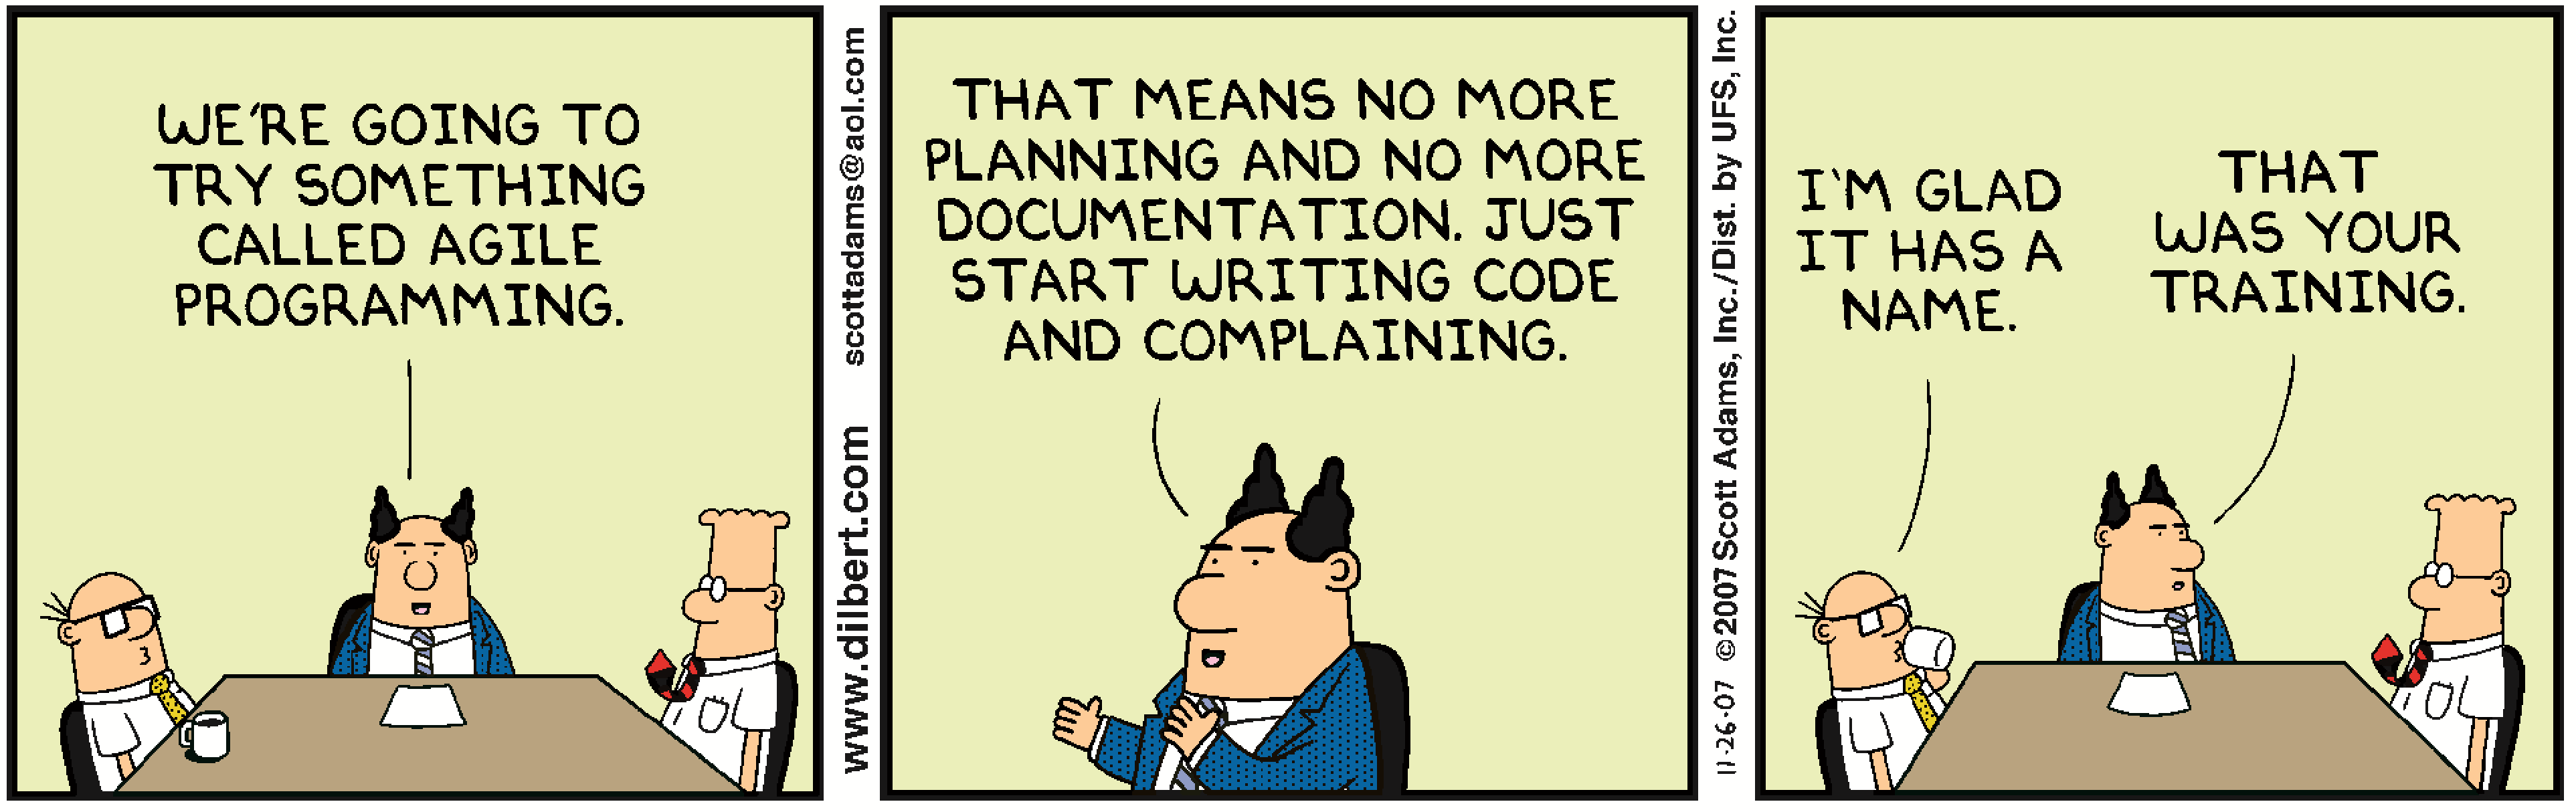
\includegraphics[width=\textwidth]{resources/Dilbert_Training_Agile_Programming}\\
		\caption{The Waterfall and Prototype SDLC models}
	\end{figure}

